\documentclass[12pt, fullpage,letterpaper]{article}

\usepackage[margin=1in]{geometry}
\usepackage{url}
\usepackage{amsmath}
\usepackage{amssymb}
\usepackage{amsfonts}
\usepackage{dsfont}
\usepackage{xspace}
\usepackage{graphicx}
\usepackage{hyperref}
\usepackage{xcolor}
\usepackage{ulem}
\usepackage{cancel}
\usepackage{float}

\newcommand\Ccancel[2][black]{\renewcommand\CancelColor{\color{#1}}\cancel{#2}}


\def\red{\color{red}}
\def\blue{\color{blue}}
\def\blackblue{\color{black!40!blue}}

\newcommand{\semester}{Spring 2022}
\newcommand{\assignmentId}{2}
\newcommand{\releaseDate}{22 Feb, 2022}
\newcommand{\dueDate}{11:59pm, 15 March, 2022}

\newcommand{\bx}{{\bf x}}
\newcommand{\bw}{{\bf w}}

\title{CS 6190: Probabilistic Machine Learning \semester}
\author{Homework \assignmentId\\
{\red Meysam Alishahi (U1323606)}}
\date{Handed out: \releaseDate\\
  Due: \dueDate}

\begin{document}
\maketitle

% Math commands by Thomas Minka
\newcommand{\var}{{\rm var}}
\newcommand{\Tr}{^{\rm T}}
\newcommand{\vtrans}[2]{{#1}^{(#2)}}
\newcommand{\kron}{\otimes}
\newcommand{\schur}[2]{({#1} | {#2})}
\newcommand{\schurdet}[2]{\left| ({#1} | {#2}) \right|}
\newcommand{\had}{\circ}
\newcommand{\diag}{{\rm diag}}
\newcommand{\invdiag}{\diag^{-1}}
\newcommand{\rank}{{\rm rank}}
% careful: ``null'' is already a latex command
\newcommand{\nullsp}{{\rm null}}
\newcommand{\tr}{{\rm tr}}
\renewcommand{\vec}{{\rm vec}}
\newcommand{\vech}{{\rm vech}}
\renewcommand{\det}[1]{\left| #1 \right|}
\newcommand{\pdet}[1]{\left| #1 \right|_{+}}
\newcommand{\pinv}[1]{#1^{+}}
\newcommand{\erf}{{\rm erf}}
\newcommand{\hypergeom}[2]{{}_{#1}F_{#2}}

% boldface characters
\renewcommand{\a}{{\bf a}}
\renewcommand{\b}{{\bf b}}
\renewcommand{\c}{{\bf c}}
\renewcommand{\d}{{\rm d}}  % for derivatives
\newcommand{\e}{{\bf e}}
\newcommand{\f}{{\bf f}}
\newcommand{\g}{{\bf g}}
\newcommand{\h}{{\bf h}}
%\newcommand{\k}{{\bf k}}
% in Latex2e this must be renewcommand
\renewcommand{\k}{{\bf k}}
\newcommand{\m}{{\bf m}}
\newcommand{\mb}{{\bf m}}
\newcommand{\n}{{\bf n}}
\renewcommand{\o}{{\bf o}}
\newcommand{\p}{{\bf p}}
\newcommand{\q}{{\bf q}}
\renewcommand{\r}{{\bf r}}
\newcommand{\s}{{\bf s}}
\renewcommand{\t}{{\bf t}}
\renewcommand{\u}{{\bf u}}
\renewcommand{\v}{{\bf v}}
\newcommand{\w}{{\bf w}}
\newcommand{\x}{{\bf x}}
\newcommand{\y}{{\bf y}}
\newcommand{\z}{{\bf z}}
%s\newcommand{\l}{\boldsymbol{l}}
\newcommand{\A}{{\bf A}}
\newcommand{\B}{{\bf B}}
\newcommand{\C}{{\bf C}}
\newcommand{\D}{{\bf D}}
\newcommand{\E}{{\bf E}}
\newcommand{\F}{{\bf F}}
\newcommand{\G}{{\bf G}}
\renewcommand{\H}{{\bf H}}
\newcommand{\I}{{\bf I}}
\newcommand{\J}{{\bf J}}
\newcommand{\K}{{\bf K}}
\renewcommand{\L}{{\bf L}}
\newcommand{\M}{{\bf M}}
\newcommand{\N}{\mathcal{N}}  % for normal density
\newcommand{\Dcal}{\mathcal{D}}  % for normal density

%\newcommand{\N}{{\bf N}}
\renewcommand{\O}{{\bf O}}
\renewcommand{\P}{{\bf P}}
\newcommand{\Q}{{\bf Q}}
\newcommand{\R}{{\bf R}}
\renewcommand{\S}{{\bf S}}
\newcommand{\T}{{\bf T}}
\newcommand{\U}{{\bf U}}
\newcommand{\V}{{\bf V}}
\newcommand{\W}{{\bf W}}
\newcommand{\X}{{\bf X}}
\newcommand{\Y}{{\bf Y}}
\newcommand{\Z}{{\bf Z}}

% this is for latex 2.09
% unfortunately, the result is slanted - use Latex2e instead
%\newcommand{\bfLambda}{\mbox{\boldmath$\Lambda$}}
% this is for Latex2e
\newcommand{\bfLambda}{\boldsymbol{\Lambda}}

% Yuan Qi's boldsymbol
\newcommand{\bsigma}{\boldsymbol{\sigma}}
\newcommand{\balpha}{\boldsymbol{\alpha}}
\newcommand{\bpsi}{\boldsymbol{\psi}}
\newcommand{\bphi}{\boldsymbol{\phi}}
\newcommand{\boldeta}{\boldsymbol{\eta}}
\newcommand{\Beta}{\boldsymbol{\eta}}
\newcommand{\btau}{\boldsymbol{\tau}}
\newcommand{\bvarphi}{\boldsymbol{\varphi}}
\newcommand{\bzeta}{\boldsymbol{\zeta}}

\newcommand{\blambda}{\boldsymbol{\lambda}}
\newcommand{\bLambda}{\mathbf{\Lambda}}
\newcommand{\bOmega}{\mathbf{\Omega}}
\newcommand{\bomega}{\mathbf{\omega}}
\newcommand{\bPi}{\mathbf{\Pi}}

\newcommand{\btheta}{\boldsymbol{\theta}}
\newcommand{\bpi}{\boldsymbol{\pi}}
\newcommand{\bxi}{\boldsymbol{\xi}}
\newcommand{\bSigma}{\boldsymbol{\Sigma}}

\newcommand{\bgamma}{\boldsymbol{\gamma}}
\newcommand{\bGamma}{\mathbf{\Gamma}}

\newcommand{\bmu}{\boldsymbol{\mu}}
\newcommand{\1}{{\bf 1}}
\newcommand{\0}{{\bf 0}}

% \newcommand{\comment}[1]{}

\newcommand{\bs}{\backslash}
\newcommand{\ben}{\begin{enumerate}}
\newcommand{\een}{\end{enumerate}}

 \newcommand{\notS}{{\backslash S}}
 \newcommand{\nots}{{\backslash s}}
 \newcommand{\noti}{{\backslash i}}
 \newcommand{\notj}{{\backslash j}}
 \newcommand{\nott}{\backslash t}
 \newcommand{\notone}{{\backslash 1}}
 \newcommand{\nottp}{\backslash t+1}
% \newcommand{\notz}{\backslash z}

\newcommand{\notk}{{^{\backslash k}}}
%\newcommand{\noti}{{^{\backslash i}}}
\newcommand{\notij}{{^{\backslash i,j}}}
\newcommand{\notg}{{^{\backslash g}}}
\newcommand{\wnoti}{{_{\w}^{\backslash i}}}
\newcommand{\wnotg}{{_{\w}^{\backslash g}}}
\newcommand{\vnotij}{{_{\v}^{\backslash i,j}}}
\newcommand{\vnotg}{{_{\v}^{\backslash g}}}
\newcommand{\half}{\frac{1}{2}}
\newcommand{\msgb}{m_{t \leftarrow t+1}}
\newcommand{\msgf}{m_{t \rightarrow t+1}}
\newcommand{\msgfp}{m_{t-1 \rightarrow t}}

\newcommand{\proj}[1]{{\rm proj}\negmedspace\left[#1\right]}
\newcommand{\argmin}{\operatornamewithlimits{argmin}}
\newcommand{\argmax}{\operatornamewithlimits{argmax}}

\newcommand{\dif}{\mathrm{d}}
\newcommand{\abs}[1]{\lvert#1\rvert}
\newcommand{\norm}[1]{\lVert#1\rVert}

%miscellaneous symbols
\newcommand{\ie}{{{i.e.,}}\xspace}
\newcommand{\eg}{{{\em e.g.,}}\xspace}
\newcommand{\EE}{\mathbb{E}}
\newcommand{\VV}{\mathbb{V}}
\newcommand{\sbr}[1]{\left[#1\right]}
\newcommand{\rbr}[1]{\left(#1\right)}
\newcommand{\cmt}[1]{}



\footnotesize
	\begin{itemize}
		\item You are welcome to talk to other members of the class about
		the homework. I am more concerned that you understand the
		underlying concepts. However, you should write down your own
		solution. Please keep the class collaboration policy in mind.
		
		\item Feel free discuss the homework with the instructor or the TAs.
		
		\item Your written solutions should be brief and clear. You need to
		show your work, not just the final answer, but you do \emph{not}
		need to write it in gory detail. Your assignment should be {\bf no
			more than 10 pages}. Every extra page will cost a point.
		
		\item Handwritten solutions will not be accepted.
		
		\item The homework is due by \textbf{midnight of the due date}. Please submit
		the homework on Canvas.
	\end{itemize}



\section*{Analytical problems [60 points + 25 bonus]}	
\label{sec:q1}
%1. show Jeffery's prior for Gaussian
%2. show Jeffern's prior for Poisson 
\begin{enumerate}
\item~[10 points] Given a Gaussian likelihood, $p(x|\mu, \sigma)=\N(x|\mu, \sigma^2)=\frac{1}{\sqrt{2\pi}\sigma}\exp\big(-\frac{1}{2\sigma^2}(x-\mu)^2\big)$,  following the general definition of Jeffery's prior, 
\begin{enumerate}
	\item~[5 points] show that given $\sigma$ fixed, the Jeffery's prior over $\mu$, $\pi_J(\mu) \propto 1$;\\
	{\bf \red Answer:}{\blackblue
	We first need to sompute Fisher information 
	\begin{align*}
	I(\mu) &= -\mathbb{E}_{\mu}\left[\frac{\d^2 \log p(x|\mu)}{\d\mu^2}\right]\\
	& = - \mathbb{E}_{\mu}\left[\frac{\d^2}{\d\mu^2}\left(C -\frac{1}{2\sigma^2}(x-\mu)^2 \right)\right]\\
	& = \mathbb{E}_{\mu}\left[\frac{1}{\sigma^2}\right] = \frac{1}{\sigma^2} .
	\end{align*}
	Therefore, since $\sigma$ is considered constant
	$\pi_J(\mu) \propto \left|\frac{1}{\sigma^2} \right|^{1/2} = \frac{1}{\sigma} \propto 1.$
	}
	\item~[5 points] show that given $\mu$ fixed, the Jeffery's prior over $\sigma$, $\pi_J(\sigma) \propto \frac{1}{\sigma}$.\\
	{\bf \red Answer:} {\blackblue
	\begin{align*}
	I(\mu) &= -\mathbb{E}_{\sigma}\left[\frac{\d^2 \log p(x|\sigma)}{\d\sigma^2}\right]\\
	& = - \mathbb{E}_{\sigma}\left[\frac{\d^2}{\d\sigma^2}\left(C -\log \sigma -\frac{1}{2\sigma^2}(x-\mu)^2 \right)\right]\\
	& = - \mathbb{E}_{\sigma}\left[\frac{1}{\sigma^2}- \frac{3}{\sigma^4}(x-\mu)^2\right]\\
	& = -\left(\frac{1}{\sigma^2} - \frac{3}{\sigma^4}\mathbb{E}_{\sigma}\left[(x-\mu)^2\right]\right) \\
	& = -\frac{1}{\sigma^2} +\frac{3}{\sigma^4} \sigma^2 = \frac{2}{\sigma^2}.
	\end{align*}
	Therefore, $\pi_J(\mu) \propto \left | \frac{2}{\sigma^2} \right|^{1/2} \propto \frac{1}{\sigma}.$
	}
\end{enumerate}

\item~[5 points] Derive the Jeffery's prior for $\lambda$ in the Poisson likelihood, $p(x=n) = e^{-\lambda}\frac{\lambda^n}{n!}$.\\
	{\bf \red Answer:} {\blackblue
	\begin{align*}
	I(\mu) &= -\mathbb{E}_{\lambda}\left[\frac{\d^2 \log p(x = n|\lambda)}{\d\lambda^2}\right]\\
	& = - \mathbb{E}_{\lambda}\left[\frac{\d^2}{\d\sigma^2}\left(-\lambda + n\log \lambda - C\right)\right]\\
	& = \mathbb{E}_{\lambda}\left[\frac{n}{\lambda^2}\right] = \frac{1}{\lambda^2} \mathbb{E}_{\lambda}\left[n\right] = \frac{1}{\lambda^2}\lambda = \frac{1}{\lambda}.
	\end{align*}
	Therefore, $\pi_J(\lambda) \propto  \left | \frac{1}{\lambda} \right|^{1/2} \propto \frac{1}{\sqrt{\lambda}}.$
	}


\item~[5 points] Given an infinite sequence of Independently Identically Distributed (IID) random variables, show that they are exchangeable.\\
	{\bf \red Answer:} {\blackblue 
	For any finite subsets $x_1,\ldots,x_n$ of these IID random variables, using Bayes rule, we have  
	\begin{align*}
	P(x_1,\ldots,x_n) & = p(x_1)p(x_2|x_1)\cdots p(x_n|x_1,\ldots,x_{n-1})\\
	& = \prod_{i=1}^n p(x_i)\quad\quad \text{since $x_i$'s are independent}
	\end{align*}
	Now, assume that $\sigma:[n]\longrightarrow [n]\in S_n$ is a permutation. Again,
	\begin{align*}
	P(x_{\sigma(1)},\ldots,x_{\sigma(n)}) 
	& = p(x_{\sigma(1)})p(x_{\sigma(2)}|x_{\sigma(1)})\cdots p(x_{\sigma(n)}|x_{\sigma(1)},\ldots,x_{\sigma(n-1)})\\
	& = \prod_{i=1}^n p(x_{\sigma(i)})\quad\quad \text{since $x_i$'s are independent and  $\sigma$ is a permutation}\\
	& = \prod_{i=1}^n p(x_i)\quad\quad \text{since $\sigma$ is a permutation }\\
	& = P(x_1,\ldots,x_n).
	\end{align*}
	}
	\vspace{-.5cm}
\item~[10 points] We discussed Polya's Urn problem as an example of exchangeability. If you do not recall, please look back at the slides we shared in the course website. Now, given  two finite sequences $(0, 1, 0, 1)$ and $(1,1, 0, 0)$,  derive their probabilities and show they are the same. \\
	{\bf \red Answer:} {\blackblue 
	\begin{align*}
	P(0, 1, 0, 1) & = p(x_1 = 0)p(x_2=1|x_1 =0)p(x_3=0|x_1= 0, x_2 = 1)p(x_4 = 1|x_1= 0, x_2 = 1, x_3 = 0, x_4 = 1)\\
	& = \frac{W_0}{B_0+W_0} \times \frac{B_0}{B_0+W_0+ a-1}\times \frac{W_0+a-1}{B_0+W_0+ 2(a-1)}\times \frac{B_0+a-1}{B_0+W_0+ 3(a-1)}\\
	& = \frac{B_0(B_0+a-1)W_0(W_0+a-1)}{\prod_{i=0}^3(B_0+W_0 + i(a-1))}
	\end{align*}
	
	\begin{align*}
	P(1, 1, 0, 0) & = p(x_1 = 1)p(x_2=1|x_1 =1)p(x_3=0|x_1= 1, x_2 = 1)p(x_4 = 0|x_1= 0, x_2 = 1, x_3 = 1, x_4 = 0)\\
	& = \frac{B_0}{B_0+W_0} \times \frac{B_0+a-1}{B_0+W_0+ (a-1)}\times \frac{W_0}{B_0+W_0+ 2(a-1)}\times \frac{W_0+a-1}{B_0+W_0+ 3(a-1)}\\
	& = \frac{B_0(B_0+a-1)W_0(W_0+a-1)}{\prod_{i=0}^3(B_0+W_0 + i(a-1))} = P(0, 1, 0, 1).
	\end{align*}
	}
\item~[10 points] For the logistic regression model, we assign a Gaussian prior over the feature weights,  $p(\w) = \N(\w|\0, \lambda\I)$. Please derive the Newton-Raphson updates. \\
	{\bf \red Answer:} {\blackblue Our objective is to find $\w$ maximizing 
	\begin{align*}
	p(\w|\t) & = p(\w) p(\t|\w,\x) = p(\w)\prod_{i=1}^n p(\t_i|\w,\x_i)\\
	& = p(\w)\prod_{i=1}^n  y_n^{t_n}(1-y_n)^{1-t_n}\quad\quad\text{where $y_n = \sigma(\w^\top \phi_n).$}
	\end{align*}
	It is equvalent to find $\w$ minimizing 
	\begin{align*}
	E(w) & = -\log p(\w|\t)\\
	& = -\log p(\w) - \sum_{i=1}^n\left(t_n\log y_n + (1-t_n)\log(1-y_n)\right)  \\
	& = C + \frac{1}{2\lambda}\w^\top\w - \sum_{i=1}^n\Big(t_n\log y_n + (1-t_n)\log(1-y_n)\Big)
	\end{align*}
	Consequently, (in details, it was computed in the class!)
	\begin{align*}
	\nabla E(\w) & =\frac{1}{\lambda}\w + \sum_{i=1}^n (y_n-t_n)\phi_n =  \frac{1}{\lambda}\w+  \bphi^\top(\y-\t)
	\end{align*}
	%where $\bphi = ???$ and ...
	Therefore, 
	\begin{align*}
	\H & = \nabla^2 E(\w) =\frac{1}{\lambda}\I_{d}+ \sum_{i=1}^n y_n(1-y_n)\phi_n\phi_n^\top\\
	& = \frac{1}{\lambda} \I_d + \bphi^\top \R\bphi,
	\end{align*}
	where $\R$ is an $n\times n$ diagonal matrix whose $(i,i)$ enrty is $y_n(1-y_n)$ and $\bphi$ is a $n\times d$ matrix whose $i$-th row is the $i$-th data point $x_i$.
	Finally, we can derive the Newton-Raphson updates as follows:
	\begin{align*}
	\w^{old} = \w^{old} - \H^{-1}\left[\frac{1}{\lambda} \w +   \bphi^\top(\y-\t)\right]
	\end{align*} 
	}
\item~[\textbf{Bonus}][20 points]  For the probit regression model, we assign a Gaussian prior over the feature weights,  $p(\w) = \N(\w|\0, \lambda\I)$. Please derive the Newton-Raphson updates. \\
	{\bf \red Answer:} {\blackblue Our objective is to find $\w$ minimizing 
	\begin{align*}
	p(\w|\t) & = p(\w) p(\t|\w,\x) = p(\w)\prod_{i=1}^n p(\t_i|\w,\x_i)\\
	& = p(\w)\prod_{i=1}^n  y_n^{t_n}(1-y_n)^{1-t_n}\quad\quad\text{where $y_n = \psi(\w^\top \phi_n)=\int_{-\infty}^{\w^\top \phi_n}\frac{1}{\sqrt{2\pi}}e^{-\frac{x^2}{2}}\d x.$}
	\end{align*}
	It is equvalent to find $\w$ maximizing 
	\begin{align*}
	E(w) & = -\log p(\w|\t)\\
	& = -\log p(\w) - \sum_{i=1}^n\left(t_n\log y_n + (1-t_n)\log(1-y_n)\right)  \\
	& = C + \frac{1}{2\lambda}\w^\top\w - \sum_{i=1}^N\Big(t_n\log y_n + (1-t_n)\log(1-y_n)\Big).
	\end{align*}
	Using the Leibniz integral rule, 
	$$\frac{\partial  y_n}{\partial \w} = \frac{1}{\sqrt{2\pi}}e^{-\frac{(\w^\top\bphi_n)^2}{2}}\phi_n,$$
	which implies  
	\begin{align*}
	\nabla E(\w) & =\frac{1}{\lambda}\w - \sum_{i=1}^N \Big(\frac{t_n}{y_n} - \frac{1-t_n}{1-y_n} \Big)\frac{\partial y_n}{\partial \w}\\
	& =  \frac{1}{\lambda}\w - \frac{1}{\sqrt{2\pi}}\sum_{i=1}^N \Big(\frac{t_n}{y_n} - \frac{1-t_n}{1-y_n} \Big)e^{-\frac{(\w^\top\bphi_n)^2}{2}}\phi_n\\
	& =  \frac{1}{\lambda}\w + \sum_{i=1}^N \underbrace{\frac{1}{\sqrt{2\pi}}\Big(\frac{y_n-t_n}{y_n(1-y_n)} \Big)e^{-\frac{(\w^\top\bphi_n)^2}{2}}}_{=z_n}\phi_n\\
	& =  \frac{1}{\lambda}\w +\bphi^\top\z,	
	\end{align*}
	where $\z$ is a $N\times 1$ vector whose $i^{th}$ entry is $z_n$. 
	Moreover, 
	\begin{align*}
	\H = \nabla\nabla E(\w) 
	& = \nabla\left( \frac{1}{\lambda}\w- \frac{1}{\sqrt{2\pi}}\sum_{n=1}^N \Big(\frac{t_n}{y_n} - \frac{1-t_n}{1-y_n} \Big)e^{-\frac{(\w^\top\phi)^2}{2}}\phi_n\right)\\
	& = \frac{1}{\lambda}\I_{d} - \frac{1}{2\pi}\sum_{n=1}^N \Big(\frac{-t_n}{y_n^2} - \frac{1-t_n}{(1-y_n)^2} \Big)e^{-(\w^\top\phi_n)^2}
	+ \frac{1}{\sqrt{2\pi}}\sum_{i=1}^N \Big(\frac{t_n}{y_n} - \frac{1-t_n}{1-y_n} \Big)(w^\top\phi_n)e^{-\frac{(\w^\top\phi)^2}{2}} \phi_n^\top\phi_n
	\\
	& = \frac{1}{\lambda}\I_{d} + \sum_{n=1}^N\left\{\underbrace{\frac{1}{2\pi} \Big(\frac{t_n}{y_n^2} + \frac{1-t_n}{(1-y_n)^2} \Big)e^{-(\w^\top\phi_n)^2}
	+ \frac{1}{\sqrt{2\pi}} \Big(\frac{-t_n}{y_n} + \frac{1-t_n}{1-y_n} \Big)(w^\top\phi_n)e^{-\frac{(\w^\top\phi)^2}{2}}}_{=r_n}\right\} \phi_n^\top\phi_n
	\\
	& = \frac{1}{\lambda}\I_{d} + \bphi^\top\R\bphi,
	\end{align*}
	where $R$ is a diagonal $N\times N$ matrix whose $(n,n)$-th value is $R_n$.
	Finally, we can derive the Newton-Raphson updates as follows:
	\begin{align*}
	\w^{old} = \w^{old} - \H^{-1}\left[\frac{1}{\lambda} \w +   \bphi^\top\z\right]
	\end{align*} 
	}
   
\item~[10 points] What are the link functions of the following models?
\begin{enumerate}
	\item~[5 points] Logistic regression
	{\bf \red Answer:} {\blackblue The Logistic regression model is a binary model in which for a feature vector $\bphi$ and a weight vector $\w$,
	\begin{align*}
	p(t|\w, \bphi) & = \sigma(\w^\top\bphi)^t\big[1-\sigma(\w^\top\bphi)\big]^{1-t},
	\end{align*}
	where $t\in\{0,1\}$. Writting $p(t|\w, \bphi)$ in a form of exponentioal family distribution member, we will have 
	\begin{align*}
	p(t|\w, \bphi)  & = \exp\Big\{t\log \sigma(\w^\top\bphi) + (1-t)\log\big(1-\sigma(\w^\top\bphi)\big)\Big\}\\
	& = \left(1-\sigma(\w^\top\bphi)\right)\exp\left\{\log\left(\frac{\sigma(\w^\top\bphi)}{1-\sigma(\w^\top\bphi)} \right)t \right\}\\
	& = \sigma(-\w^\top\bphi)\exp\left\{(\w^\top\bphi)t \right\}\\
	& \exp\left\{(\w^\top\bphi)t -\log \sigma(-\w^\top\bphi) \right\}
	\end{align*}
	Comparison to the sandard form of exponentioal family distribution
	$$p(t|\eta) = h(t)\exp\left\{\eta t - g(\eta)\right\},$$
	we obtain 
	$$\u(t) = t\quad \quad h(t) =1 \quad\quad \eta =  \w^\top\bphi \quad\quad \mbox{and} \quad\quad g(\eta) =-\log(\sigma(-\eta)).$$
	Therefore, 
	\begin{align*}
	y = \EE_\eta(t|\eta) & = \frac{\partial g(\eta)}{\partial \eta}\\
	& = \frac{\sigma(-\eta)(1-\sigma(-\eta))}{\sigma(-\eta)}\\
	& = 1-\sigma(-\eta) = \sigma(\eta)
	\end{align*}
	which implies $\eta = \sigma^{-1}(y) = \log(\frac{y}{1-y})$ is the link function. 
	}
	\item~[5 points] Poisson regression: $p(x=n) = e^{-\lambda}\frac{\lambda^n}{n!}$ where $\lambda = \w^\top \bphi$. 
	{\bf \red Answer:} {\blackblue 
	Rewritting Poisson distributions in the form of exponentioal family distributions, we obtain
	\begin{align*}
	p(x=n|\w,\phi) & = e^{-\lambda}\frac{\lambda^n}{n!} = \frac{1}{n!}\exp\left\{ n\log\lambda-\lambda\right\}.
	\end{align*}
	Therefore, 
	$$h(x) = \frac{1}{x!} \quad\quad \u(x) =x \quad\quad \eta = \log \lambda=\log \w^\top\bphi\quad\quad \mbox{and}\quad\quad g(\eta) = \lambda = e^\eta = \w^\top\bphi.$$
	Accordingly, 
	$y = \EE_\eta(x|\eta) = \frac{\partial g(\eta)}{\partial \eta} = e^\eta = \w^\top\bphi$
	which implies $\eta = \log y$ is the link function. 
	}
\end{enumerate}

\item~[10 points] As we discussed in the class, the probit regression model is equivalent to given each feature vector $\bphi$, sampling a latent variable $z$ from $\N(z|\w^\top \bphi,1)$,  and then sampling the binary label $t$ from the step distribution, $p(t|z) = \mathds{1}(t=0)\mathds{1}(z< 0) + \mathds{1}(t=1)\mathds{1}(z\ge 0)$ where $\mathds{1}(\cdot)$ is the indicator function. Show that if we marginalize out $z$, we recover the original likelihood of the probit regression.  \\
	{\bf \red Answer:} {\blackblue 
	\begin{align*}
	p(t|\phi) & = \int_{-\infty}^{+\infty} p(t,z|\w,\bphi)\d z =  \int_{-\infty}^{+\infty} p(z|\w,\bphi)p(t|z)\d z\\
	& = \int_{-\infty}^{+\infty} \N(z|\w^\top \bphi,1)\Big[\mathds{1}(t=0)\mathds{1}(z\leq 0) + \mathds{1}(t=1)\mathds{1}(z\geq 0)\Big]\d z\\
	& = \mathds{1}(t=0)\int_{-\infty}^{0} \N(z|\w^\top \bphi,1) \d z + \mathds{1}(t=1)\int_{0}^{+\infty} \N(z|\w^\top \bphi,1)\d z\\
	& = \mathds{1}(t=0)\int_{-\infty}^{-w^\top \bphi} \N(u|\0,1) \d u + \mathds{1}(t=1)\int_{-w^\top \bphi}^{+\infty} \N(u|0,1)\d u\quad\quad\mbox{ changing variable $u = z-w^\top \bphi$}\\
	& = \mathds{1}(t=0)(1-\psi(\w^\top \bphi)) + \mathds{1}(t=1)\left[\psi(\w^\top \bphi)\right] \quad\quad\mbox{symetry of Normal distribution}\\
	& = \psi(\w^\top \bphi)^t\big(1-\psi(\w^\top \bphi)\big)^{1-t}.
	\end{align*}
	}
\vspace{-.5cm}
\item~[\textbf{Bonus}][5 points] For polynomial regression (1d feature vector), show that given $N$ training points, you can always choose the highest order $M$ for the polynomial terms such that your model results in $0$ training error (\eg mean squared error or mean absolute error).  Please give the corresponding regression function as well. 
	{\bf \red Answer:} {\blackblue Assume that our data set is $\{(x_1,y_1),\ldots,(x_N,y_N)\}$. 
	Define $$P(x) = \sum_{i=1}^Ny_i \underbrace{\prod_{j=1, j\neq i}^N\frac{x-x_j}{x_i-x_j}}_{=Q_i(x)}$$
	Note that for each $i,k\in[N]$,  
	$$Q_i(x_k) =\left\{
	\begin{array}{cc}
	0 & i\neq k\\
	1 & i=k.
	\end{array}\right.$$
	Thus, for each $k\in[N]$, 
	$P(x_k) = \sum_{i=1}^Ny_i Q_i(x_k) = y_k.$
	Accordingly, $P(x)$ is a polynomial of degree $N-1$ which perfectly fits the data. 
	} 
\end{enumerate}

\section*{Practice [40 points + 45 Bonus]}
\begin{enumerate}
	\item~[15 Points] Let us generate a simulation dataset for fun. We consider a linear regression model $y(\x, \w) = w_0 + w_1 x$. We set the ground-truth $w_0 = -0.3$ and $w_1 = 0.5$. We generate $20$ samples $[x_1, \ldots, x_{20}]$ from the uniform distribution in $[-1, 1]$. For each sample $x_n$, we obtain an sample $y_n$ by first calculating $w_0 + w_1 x_n$ with the ground-truth values of $w_0$ and $w_n$, and then adding a Gaussian noise with zero mean, standard deviation $0.2$. Now let us verify what we have discussed in the class. We use a Bayesian linear regression model. The prior of $\w$ is $\N(\w|\0, \alpha \I)$, and the likelihood for each sample is $p(y_n|\x_n, \w) = \N(y_n|w_0 + w_1x, \beta^{-1}\I)$. Here we set $\alpha = 2$ and $\beta = 25$. 
	\begin{enumerate}
		\item~[3 points] Draw the heat-map of the prior $p(\w)$ in the region $w_0 \in [-1, 1]$ and $w_1 \in [-1, 1]$, where you represent the values of $p(\w)$ for different choices of $\w$ with different colors. The darker some given color (\eg red), the larger the value; the darker some the other given color (\eg blue), the smaller the value.  Most colors should be in between. Then sample $20$ instances of $\w$ from $p(\w)$. For each $w$, draw a line $y = w_0 + w_1x$ in the region $x, y \in [-1, 1]$. Ensure these $20$ lines are in the same plot. What do you observe?\\
	{\bf \red Answer:} {\blackblue 
	The prior contours are circles as it is a Gaussian distribution with zero mean and multiplication of identity matrix as its covariance matrix. 
	Also, in the region we plot the 20 lines, these lines seems have be completely random slopes.  
	\begin{figure}[H]
	\begin{center}
	\begin{minipage}{0.45\textwidth}
     	\frame{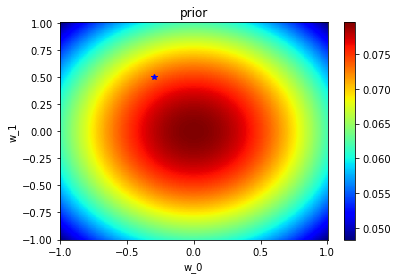
\includegraphics[width=0.85 \linewidth]{Images/prior.png}}
     	\caption{{\footnotesize Prior}}\label{Fig.2}      
 	\end{minipage}
 	\begin{minipage}{0.45\textwidth}
     	\frame{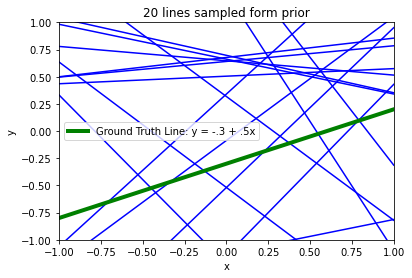
\includegraphics[width=0.85 \linewidth]{Images/line_prior.png}}
     	\caption{{\footnotesize 20 lines whose coefficients are sampled from prior}}\label{Fig.2}      
 	\end{minipage}
	 \end{center}
	\end{figure}
	}	
		\item~[3 points] Calculate and report the posterior distribution of $\w$ given $(\x_1, y_1)$. Now draw the heat map of the distribution. Also draw the ground-truth of $w_0$ and $w_1$ in the heat map.  Then from the posterior distribution, sample $20$ instances of $\w$, for each of which draw a line  $y = w_0 + w_1x$ in the region $x, y \in [-1, 1]$. Ensure these 20 lines are in the same plot. Also draw $(x_1, y_1)$ as a circle in that plot. What do you observe? Why?\\
	{\bf \red Answer:} {\blackblue 
	The posterior distribution is gaussian distribution $\N(\bmu, \bSigma)$, where 
	$$\bmu =  [-0.09630267, -0.01547873]\quad\quad\text{and}\quad \quad \bSigma = \left[\begin{array}{cc}0.03684579 & -0.02622379\\
	-0.02622379 & 0.19578505
	\end{array}\right].$$
	
	The posterior distribution is more concentrated compared to prior distribution and moreover, 
	its contours are ellipsoid affected by the observed data point $(x_1,y_1)$. 
	Also, the $20$ sample lines all are tend to pass through to the data point $(x_1,y_1)$, they all pass close to this point. 
	\begin{figure}[H]
	\begin{center}
	\begin{minipage}{0.45\textwidth}
     	\frame{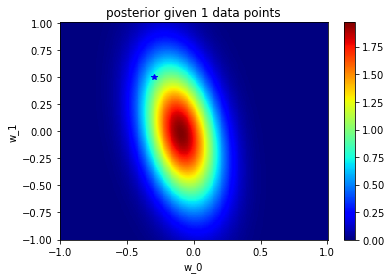
\includegraphics[width=0.85 \linewidth]{Images/posterior_1.png}}
     	\caption{{\footnotesize Posterior distribution given $(x_1,y_1)$}}\label{Fig.2}      
 	\end{minipage}
 	\begin{minipage}{0.45\textwidth}
     	\frame{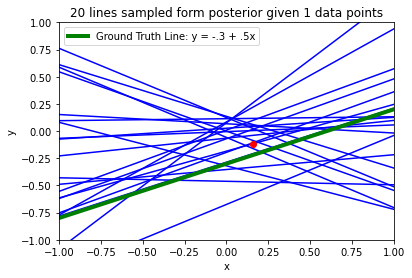
\includegraphics[width=0.85 \linewidth]{Images/line_posterior_1.png}}
     	\caption{{\footnotesize 20 lines whose coefficients are sampled from posterior given $(x_1,y_1)$}}\label{Fig.2}      
 	\end{minipage}
	 \end{center}
	\end{figure}
		
		
	}
		\item~[3 points] Calculate and report the posterior distribution of $\w$ given $(\x_1, y_1)$ and $(\x_2, y_2)$. Then draw the plots as the above. What do you observe now?  \\
	{\bf \red Answer:} {\blackblue 
	The posterior distribution is gaussian distribution $\N(\bmu, \bSigma)$, where 
	$$\bmu =  [-0.05922021, 0.20500141]\quad\quad\text{and}\quad \quad \bSigma = \left[\begin{array}{cc}0.03430475 & -0.04133198\\
	-0.04133198 & 0.10595668
	\end{array}\right].$$
		
	The posterior mean is getting closer to the ground truth $(-0.3,0.5)$ and it is now even more concentrated compared to the previous step because of the observed data points $(x_1,y_1), (x_2,y_2)$. 
	The $20$ sample lines all tend to pass through to the two data points $(x_1,y_1), (x_2,y_2)$, they all pass close these points. Also, these lines are now somehow concentrated around the ground truth line. 
	
	\begin{figure}[H]
	\begin{center}
	\begin{minipage}{0.45\textwidth}
     	\frame{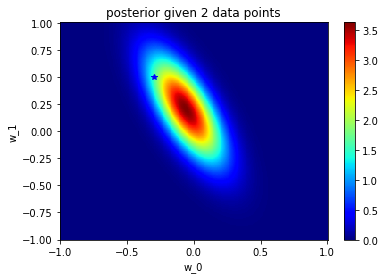
\includegraphics[width=0.95 \linewidth]{Images/posterior_2.png}}
     	\caption{{\footnotesize Posterior distribution given $(x_1,y_1)$ and $(x_2,y_2)$}}\label{Fig.2}      
 	\end{minipage}
 	\begin{minipage}{0.45\textwidth}
     	\frame{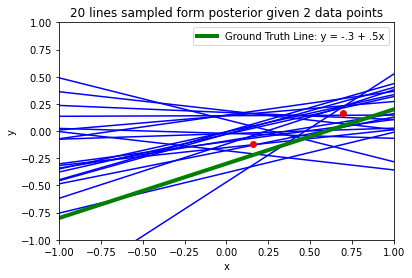
\includegraphics[width=0.95 \linewidth]{Images/line_posterior_2.png}}
     	\caption{{\footnotesize 20 lines whose coefficients are sampled from from posterior given $(x_1,y_1)$ and $(x_2,y_2)$}}\label{Fig.2}      
 	\end{minipage}
	 \end{center}
	\end{figure}
		
		
	}
		\item~[3 points] Calculate and report the posterior distribution of $\w$ given $\{(\x_1, y_1), \ldots, (\x_5, y_5)\}$. Then draw the plots as the above. What do you observe now? \\
	{\bf \red Answer:} {\blackblue 
	The posterior distribution is gaussian distribution $\N(\bmu, \bSigma)$, where 
	$$\bmu =  [-0.14286727, 0.42610391]\quad\quad\text{and}\quad \quad \bSigma = \left[\begin{array}{cc}0.00817504 & -0.00511181\\
	-0.00511181 & 0.05413014
	\end{array}\right].$$
		
	Similarly, the posterior mean is getting, even more, closer to the ground truth $(-0.3,0.5)$ and it is now even more concentrated compared to the previous step because of the observed data points $(x_1,y_1),\ldots, (x_5,y_5)$. The $20$ sample lines are now really concentrated around the ground truth line.	
	
	\begin{figure}[H]
	\begin{center}
	\begin{minipage}{0.45\textwidth}
     	\frame{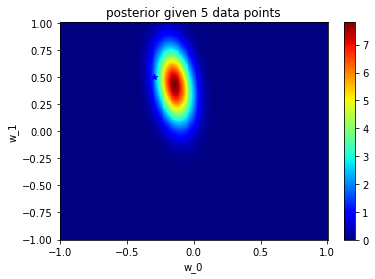
\includegraphics[width=0.95 \linewidth]{Images/posterior_5.png}}
     	\caption{{\footnotesize Posterior distribution given $\{(\x_1, y_1), \ldots, (\x_5, y_5)\}$}}\label{Fig.2}      
 	\end{minipage}
 	\begin{minipage}{0.45\textwidth}
     	\frame{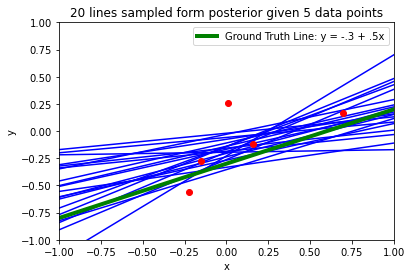
\includegraphics[width=0.95 \linewidth]{Images/line_posterior_5.png}}
     	\caption{{\footnotesize 20 lines whose coefficients are sampled from posterior given $\{(\x_1, y_1), \ldots, (\x_5, y_5)\}$}}\label{Fig.2}      
 	\end{minipage}
	 \end{center}
	\end{figure}
		
		
	}
		\item~[3 points] Calculate and report the posterior distribution of $\w$ given all the $20$ data points. Then draw the plots as the above. What do you observe now?  \\
	{\bf \red Answer:} {\blackblue 
	The posterior distribution is gaussian distribution $\N(\bmu, \bSigma)$, where 
	$$\bmu =  [-0.23654566, 0.45238796]\quad\quad\text{and}\quad \quad \bSigma = \left[\begin{array}{cc}0.00204578 &  -0.00065104\\
	-0.00065104 & 0.00646252
	\end{array}\right].$$
	
	Similarly, the posterior mean is now really close to the ground truth $(-0.3,0.5)$ and posterior is now very concentrated around its mean because of the observed data points $(x_1,y_1),\ldots, (x_{20},y_{20})$. The $20$ sample lines are now completely concentrated around the ground truth line. Indeed, each of them can be a very good approximation of the ground truth line. 
		
	\begin{figure}[H]
	\begin{center}
	\begin{minipage}{0.45\textwidth}
     	\frame{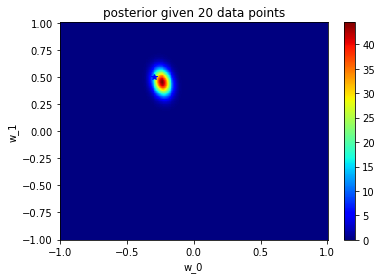
\includegraphics[width=0.95 \linewidth]{Images/posterior_20.png}}
     	\caption{{\footnotesize Posterior distribution given all the $20$ data points}}\label{Fig.2}      
 	\end{minipage}
 	\begin{minipage}{0.45\textwidth}
     	\frame{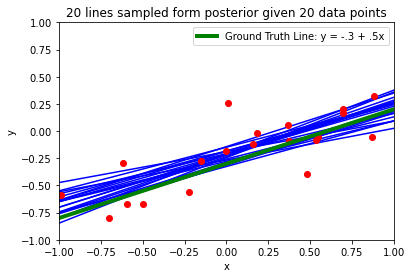
\includegraphics[width=0.95 \linewidth]{Images/line_posterior_20.png}}
     	\caption{{\footnotesize 20 lines whose coefficients are sampled from posterior given all the $20$ data points}}\label{Fig.2}      
 	\end{minipage}
	 \end{center}
	\end{figure}
		
		
	}
	\end{enumerate}
	
	\item~[25 points] We will implement  Logistic regression and Probit regression for a binary classification task --- bank-note authentication. Please download the data ``bank-note.zip'' from Canvas. The features and labels are listed in the file ``bank-note/data-desc.txt''. The training data are stored in the file ``bank-note/train.csv'', consisting of $872$ examples. The test data are stored in ``bank-note/test.csv'', and comprise of $500$ examples. In both the training and testing datasets, feature values and labels are separated by commas. To ensure numerical stability and avoid overfitting, we assign the feature weights a standard normal prior $\N(\0, \I)$.  
	\begin{enumerate}

	\item~[15 points] Implement Newton-Raphson scheme to find the MAP estimation of the feature weights in the logistic regression model. Set the maximum number of iterations to $100$ and the tolerance level to be $1e-5$,  \ie when the norm of difference between the weight vectors after one update is below the tolerance level, we consider it converges and stop updating the weights any more. Initially, you can set all the weights to be zero. Report the prediction accuracy on the test data. Now set the initial weights values be to be randomly generated, say, from the standard Gaussian, run and test your algorithm. What do you observe? Why? \\
	{\bf \red Answer:} {\blackblue 
	Prediction accuracy on the test data when we initiated all the weights to be zero is 99\%.
	 But when the values of the initial weights are randomly generated from the standard Gaussian $\N(\0, \I)$, the model is unstable and the accuracy sometimes drops down to even $50\%$ and sometimes we get the same accuracy of 99\%. The reason might be that when we randomly generate $w$, it is possible that $|w^\top\phi_n |$ is a large number (for example more than $10$) which makes either $y_n =0$ or $y_n= 1$. This vanishes the gradient since the sigmoid function has almost zero gradients for numbers with large absolute values. It causes almost no meaningful updates to $w$.  We tried some ideas to overcome this issue. First, we randomly generated $w$ from the standard Gaussian with zero mean and $10^{-5}\I$ covariance. This method works almost all the time. The other idea is that, since multiplicating $w$ by a positive number has no effect on the model accuracy, during training we can always keep tracking the $L_2$-norm of $w$ and when it is larger than $1$, we can project it on the unit ball.  This method works pretty well.
}
	\item~[10 points]  Implement MAP estimation algorithm for Probit regression model. You can calculate the gradient and feed it to any optimization algorithm, say, L-BFGS. Set the maximum number of iterations to $100$ and the tolerance level to $1e-5$. Initially, you can set all the weights to zero. Report the prediction accuracy  on the test data. Compared with logistic regression, which one is better? 
	Now set the initial weights values be to be randomly generated, say, from the standard Gaussian, run and test your algorithm. What do you observe? Can you guess why?  \\
	{\bf \red Answer:} {\blackblue 
	The prediction accuracy on the test data when we initiated all the weights to be zero is 98.8\%. 
	Compared with the logistic regression model, we can conclude that the logistic regression performs a bit better rather than Probit regression model.
	Using L-BFGS, it seems that the model is stable even when we randomly initiate $w$ where we obtain the same accuracy of 98.8\%.
	Probably, since L-BFGS is a built-in model, it takes care of the problems we encountered in the previous part. 
	}
	\item~[\textbf{Bonus}][15 points]. Implement Newton-Raphson scheme to find the MAP estimation for Probit regression. Report the prediction accuracy.\\
	{\bf \red Answer:} {\blackblue We implimented  Newton-Raphson scheme. 
	The prediction accuracy on the test data when we initiated all the weights to be zeros is 98.8\% (see the end of uploaded file HW2Q2.ipynb). 
	Again here we check the randomized initialization and we have some sort of the problems we described in Part(a).  Here also computing the Hessian matrix is numerically unstable since we have $y_n$ and $1-y_n$ in the denominator and when the initial weights are random, as described in Part (a), most likely either $y_n=0$ or $y_n =1$. However, using the same methods as described in Part (a), we could get a stable model resulting in the same accuracy of 98.8\%.
	}
	
\end{enumerate}

	
	\item~[\textbf{Bonus}][30 points]  We will implement a multi-class logistic regression model for car evaluation task. The dataset is from UCI repository(\url{https://archive.ics.uci.edu/ml/datasets/car+evaluation}). Please download the processed dataset (car.zip) from Canvas.  In this task, we have $6$ car attributes, and the label is the evaluation of the car. The attribute and label values are listed in the file ``data-desc.txt". All the attributes are categorical. Please convert each categorical attribute into binary features. For example, for ``safety: low, med, high'', we convert it into three binary features: ``safety'' is ``low'' or not, ``safety'' is ``med'' or not, and ``safety'' is  ``high'' or not. 
	The training data are stored in the file ``train.csv'', consisting of $1,000$ examples. The test data are stored in ``test.csv'', and comprise $728$ examples. In both training and test datasets, attribute values are separated by commas; the file ``data-desc.txt''  lists the attribute names in each column.  To ensure numerical stability and avoid overfitting, we assign the feature weights a standard normal prior $\N(\0, \I)$.  
	\begin{enumerate}
		\item~[15 points] Implement MAP estimation algorithm for multi-class logistic regression model. To do so, you can calculate the gradient and feed it to some optimization package, say, L-BFGS. Report the prediction accuracy on the test data. \\
	{\bf \red Answer:} {\blackblue 
	Using gradient descent to train, either with zero or random initialization, the prediction accuracy on the test data is: 91.7\%. 
	Also, using L-BFGS method, either with zero or random initialization, the prediction accuracies on the test data are: 90.7\% and 90.1\% respectively.
	
	}
		\item~[15 points] Let us use an ``ugly'' trick to convert the multi-class classification problem into a binary classification problem.
		Let us train four logistic regression models, where each model predicts one particular label, \ie ``unacc" or not, ``acc'' or not, ``good'' or not, 
		and ``vgood'' or not. Then for each test example, we run the models to get four logistic scores, \ie the probability that each label is one. 
		We choose the label with the highest score as the final prediction. Report the prediction accuracy on the test data. 
		As compared with multi-class logistic regression,which one is better? \\
	{\bf \red Answer:} {\blackblue 
	Using gradient descent to train, either with zero or random initialization, the prediction accuracy on the test data is : 85.3\%. 
	However, we need to initiate the random weights to be very small, say from $\N(0,10^{-4})$.
	
	Also, using L-BFGS method, either with zero or random initialization, the prediction accuracy on the test data is : 86.1\%.
	} 
	\end{enumerate}
	
	
	

	
\end{enumerate}
\end{document}
%%% Local Variables:
%%% mode: latex
%%% TeX-master: t
%%% End:
